\subsection{Actuators}

    \subsubsection{Thrusters}
        https://www.cubesatshop.com/wp-content/uploads/2017/04/ENP-IFM-Nano-Thruster-Product-Overview.pdf
        https://blog.satsearch.co/2019-07-10-cubesat-thrusters-an-overview-of-in-space-propulsion-products-for-small-satellites

        Parameters:
            Thrust range;
            Nominal thrust: (find a way to model change?)
            Specific impulse (also ranges?)
            Max propellant
            Total impulse
            Power (at nominal thrust?)
            Mass
            Dimensions?
            Hot standby Power
            Time delay to control
            In both directions? 

        % Bang-bang: https://apps.dtic.mil/dtic/tr/fulltext/u2/a291803.pdf
        % /resources/noise_description.pdf

        \begin{figure}[hb]
            \centering
            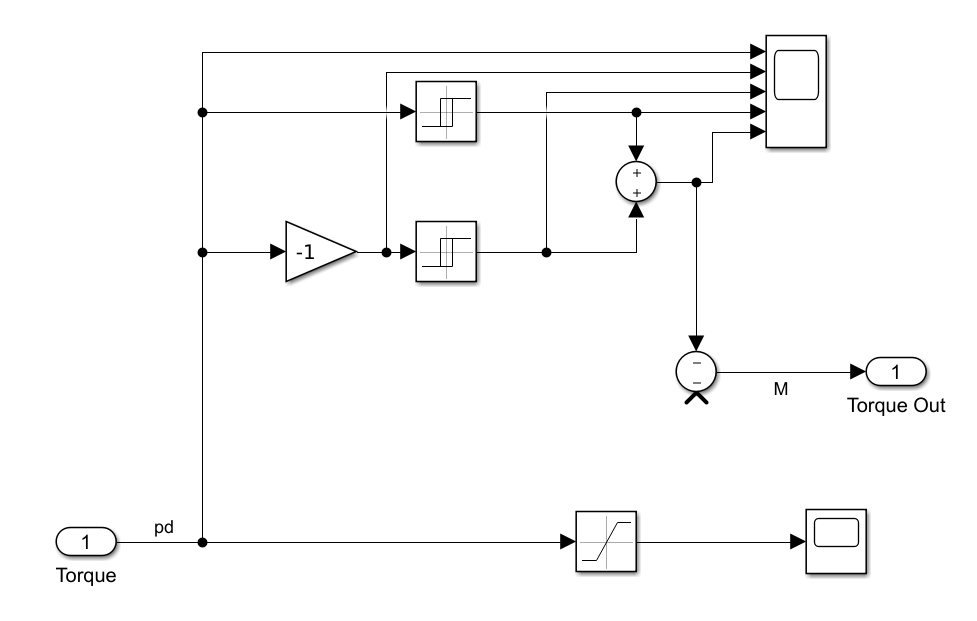
\includegraphics[width=1\textwidth]{2-toolbox/thru_simulink.png}
            \caption{Simulink Thrusters model}
            \label{fig:thru_simulink}
            Thrusters parameters: 
        \end{figure}

    \subsubsection{Reaction Wheels}
        Ideal to real: Bearing Noise, Transport Delay, Saturation, Quantization.
        
        \begin{figure}[hb]
            \centering
            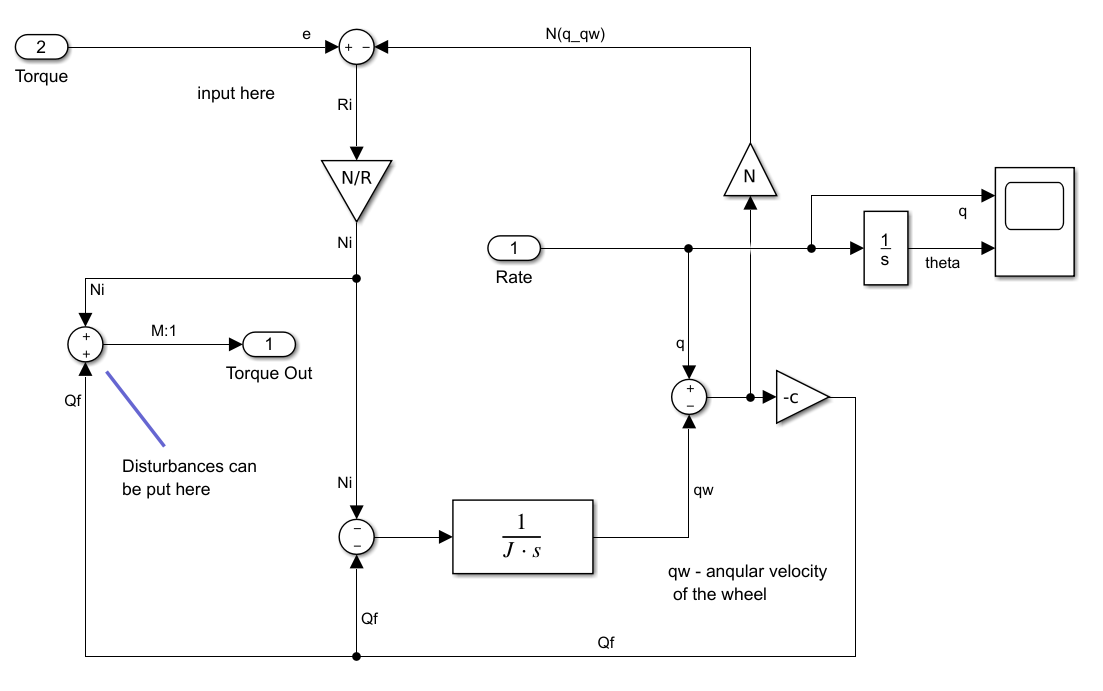
\includegraphics[width=1\textwidth]{2-toolbox/rw_simulink.png}
            \caption{Simulink Reaction Wheels model}
            \label{fig:rw_simulink}
        \end{figure}
        \subsubsection{Gimbaled Momentum Wheel}